% Transformaciones gauge en GDL
% Compilar con: pdflatex gauge_transformation.tex
\documentclass[tikz,border=10pt]{standalone}
\usepackage{tikz}
\usepackage{amsmath}
\usetikzlibrary{arrows.meta, positioning, shapes.geometric}

\definecolor{gdlblue}{RGB}{41, 98, 168}
\definecolor{gdlred}{RGB}{191, 49, 49}
\definecolor{gdlgreen}{RGB}{30, 130, 76}
\definecolor{gdlorange}{RGB}{217, 130, 30}
\definecolor{gdlpurple}{RGB}{118, 56, 138}
\definecolor{gdlgray}{RGB}{140, 140, 140}
\definecolor{gdlyellow}{RGB}{190, 140, 10}

\begin{document}
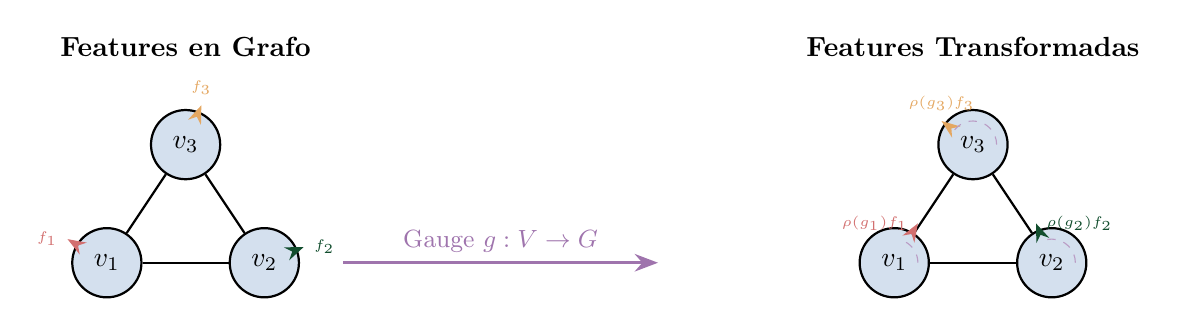
\begin{tikzpicture}[
    >=Stealth,
    vertex/.style={circle, draw, thick, minimum size=25pt},
    arrow/.style={->, thick}
]

% === Grafo con features ===
\begin{scope}[shift={(-5, 2)}]
    \node[above, font=\bfseries] at (1, 2.5) {Features en Grafo};

    % Vértices con vectores de features
    \node[vertex, fill=gdlblue!20] (a) at (0, 0) {$v_1$};
    \node[vertex, fill=gdlblue!20] (b) at (2, 0) {$v_2$};
    \node[vertex, fill=gdlblue!20] (c) at (1, 1.5) {$v_3$};

    % Aristas
    \draw[thick] (a) -- (b);
    \draw[thick] (b) -- (c);
    \draw[thick] (c) -- (a);

    % Vectores de features
    \draw[->, thick, gdlred!70] (a) -- ++(-0.5, 0.3) node[left, font=\tiny] {$f_1$};
    \draw[->, thick, gdlgreen!60!black] (b) -- ++(0.5, 0.2) node[right, font=\tiny] {$f_2$};
    \draw[->, thick, gdlorange!70] (c) -- ++(0.2, 0.5) node[above, font=\tiny] {$f_3$};
\end{scope}

% === Transformación gauge ===
\draw[->, very thick, gdlpurple!70] (-2, 2) -- node[above, font=\small] {Gauge $g: V \to G$} (2, 2);

% === Grafo transformado ===
\begin{scope}[shift={(5, 2)}]
    \node[above, font=\bfseries] at (1, 2.5) {Features Transformadas};

    % Vértices
    \node[vertex, fill=gdlblue!20] (a2) at (0, 0) {$v_1$};
    \node[vertex, fill=gdlblue!20] (b2) at (2, 0) {$v_2$};
    \node[vertex, fill=gdlblue!20] (c2) at (1, 1.5) {$v_3$};

    % Aristas
    \draw[thick] (a2) -- (b2);
    \draw[thick] (b2) -- (c2);
    \draw[thick] (c2) -- (a2);

    % Vectores rotados localmente
    \draw[->, thick, gdlred!70] (a2) -- ++(0.3, 0.5) node[left, font=\tiny] {$\rho(g_1)f_1$};
    \draw[->, thick, gdlgreen!60!black] (b2) -- ++(-0.2, 0.5) node[right, font=\tiny] {$\rho(g_2)f_2$};
    \draw[->, thick, gdlorange!70] (c2) -- ++(-0.4, 0.3) node[above, font=\tiny] {$\rho(g_3)f_3$};

    % Indicadores de rotación local
    \draw[dashed, gdlpurple!50] (a2) ++(0.3, 0) arc (0:60:0.3cm);
    \draw[dashed, gdlpurple!50] (b2) ++(0.3, 0) arc (0:120:0.3cm);
    \draw[dashed, gdlpurple!50] (c2) ++(0.3, 0) arc (0:150:0.3cm);
\end{scope}

\end{tikzpicture}
\end{document}
